\documentclass[11pt]{amsart}
%prepared in AMSLaTeX, under LaTeX2e
\addtolength{\oddsidemargin}{-.9in} 
\addtolength{\evensidemargin}{-.9in}
\addtolength{\topmargin}{-.9in}
\addtolength{\textwidth}{1.5in}
\addtolength{\textheight}{1.5in}

\renewcommand{\baselinestretch}{1.05}

\usepackage{verbatim} % for "comment" environment

\usepackage{palatino}

\usepackage[final]{graphicx}

\usepackage{tikz}
\usetikzlibrary{positioning}

\usepackage{enumitem,xspace,fancyvrb}
\usepackage[pdftex,colorlinks=true]{hyperref}

\newtheorem*{thm}{Theorem}
\newtheorem*{defn}{Definition}
\newtheorem*{example}{Example}
\newtheorem*{problem}{Problem}
\newtheorem*{remark}{Remark}

\DefineVerbatimEnvironment{mVerb}{Verbatim}{numbersep=2mm,frame=lines,framerule=0.1mm,framesep=2mm,xleftmargin=4mm,fontsize=\footnotesize}

% macros
\usepackage{amssymb}
\newcommand{\bA}{\mathbf{A}}
\newcommand{\bB}{\mathbf{B}}
\newcommand{\bE}{\mathbf{E}}
\newcommand{\bF}{\mathbf{F}}
\newcommand{\bJ}{\mathbf{J}}

\newcommand{\bb}{\mathbf{b}}
\newcommand{\br}{\mathbf{r}}
\newcommand{\bv}{\mathbf{v}}
\newcommand{\bw}{\mathbf{w}}
\newcommand{\bx}{\mathbf{x}}

\newcommand{\hbi}{\mathbf{\hat i}}
\newcommand{\hbj}{\mathbf{\hat j}}
\newcommand{\hbk}{\mathbf{\hat k}}
\newcommand{\hbn}{\mathbf{\hat n}}
\newcommand{\hbr}{\mathbf{\hat r}}
\newcommand{\hbt}{\mathbf{\hat t}}
\newcommand{\hbx}{\mathbf{\hat x}}
\newcommand{\hby}{\mathbf{\hat y}}
\newcommand{\hbz}{\mathbf{\hat z}}
\newcommand{\hbphi}{\mathbf{\hat \phi}}
\newcommand{\hbtheta}{\mathbf{\hat \theta}}
\newcommand{\complex}{\mathbb{C}}
\newcommand{\ppr}[1]{\frac{\partial #1}{\partial r}}
\newcommand{\ppt}[1]{\frac{\partial #1}{\partial t}}
\newcommand{\ppx}[1]{\frac{\partial #1}{\partial x}}
\newcommand{\ppy}[1]{\frac{\partial #1}{\partial y}}
\newcommand{\ppz}[1]{\frac{\partial #1}{\partial z}}
\newcommand{\pptheta}[1]{\frac{\partial #1}{\partial \theta}}
\newcommand{\ppphi}[1]{\frac{\partial #1}{\partial \phi}}
\newcommand{\Div}{\ensuremath{\nabla\cdot}}
\newcommand{\Curl}{\ensuremath{\nabla\times}}
\newcommand{\curl}[3]{\ensuremath{\begin{vmatrix} \hbi & \hbj & \hbk \\ \partial_x & \partial_y & \partial_z \\ #1 & #2 & #3 \end{vmatrix}}}
\newcommand{\cross}[6]{\ensuremath{\begin{vmatrix} \hbi & \hbj & \hbk \\ #1 & #2 & #3 \\ #4 & #5 & #6 \end{vmatrix}}}
\newcommand{\eps}{\epsilon}
\newcommand{\grad}{\nabla}
\newcommand{\ip}[2]{\ensuremath{\left<#1,#2\right>}}
\newcommand{\lam}{\lambda}
\newcommand{\lap}{\triangle}

\newcommand{\Null}{\operatorname{null}}
\newcommand{\rank}{\operatorname{rank}}
\newcommand{\range}{\operatorname{range}}
\newcommand{\trace}{\operatorname{tr}}

\newcommand{\RR}{\mathbb{R}}
\newcommand{\ZZ}{\mathbb{Z}}

\newcommand{\prob}[1]{\bigskip\bigskip\noindent\textbf{#1.}\quad }
\newcommand{\epart}[1]{\bigskip\noindent\textbf{(#1)}\quad }
\newcommand{\ppart}[1]{\,\textbf{(#1)}\quad }

\newcommand{\Matlab}{\textsc{Matlab}\xspace}
\newcommand{\ds}{\displaystyle}


\begin{document}
\scriptsize \noindent Math 252 Calculus II (Bueler) \hfill 9 December 2022 \fbox{\emph{Not turned in!}}
\normalsize\medskip

\Large\centerline{\textbf{PRACTICE Final Exam}}
\medskip
\normalsize

\thispagestyle{empty}
\begin{quote}
\emph{This practice exam is shortened to 2 pages to create a worksheet.  It is based on an old Final Exam from Fall 2020.  Full solutions are posted on the ``Exams'' tab:}

\centerline{\href{https://bueler.github.io/calc2/assets/exams/F20/final-solns.pdf}{\texttt{bueler.github.io/calc2/assets/exams/F20/final-solns.pdf}}}

\noindent \emph{Certain problem numbers are missing below because they are \emph{not} problems which could appear on our Final Exam.}

\emph{Please see the Spring 2022 Final Exam on the ``Exams'' tab.  It is the most representative!}
\end{quote}

\prob{1}  A parametric curve is given by $\ds x(t)=t^2-2t+3$, $\ds y(t)=t^3-4t$ for $-\infty<t<\infty$.

\epart{a}  Find the slope of the tangent line to the curve at the point where $t=0$.

\epart{b}  Give the $x$- and $y$-coordinates of all points on the curve where the tangent line is vertical.

\prob{2} The region bounded by the graphs of $y=4-x^2$ and $y=0$ is rotated about a vertical axis at $x=3$.  Give, by \textbf{do not evaluate}, an integral calculating the volume.

\noindent (\emph{I would not ask this because we only practiced with $x=0$ and $y=0$ axes.  Can you do it anyway?})

\prob{3}  Compute the following, showing your work.

\epart{a}  $\ds \int \frac{1}{(x^2+4)^{3/2}}\,dx$

\epart{b}  $\ds \int_0^{\pi/4} \tan^4 x \sec^4 x\,dx$

\epart{c}  $\ds \int \frac{1}{x^2-2x}\,dx$

\epart{d}  $\ds \int_0^1 \frac{1}{x^{3/2}}\,dx$

\epart{e}  $\ds \int x \ln x\,dx$

\prob{5}  An elevated water tank is shaped like a paraboloid, obtained by rotating about the $y$-axis the region bounded by that axis, the curve $y=9+x^2$ for $x\ge 0$, and the line $y=18$.  Both $x$ and $y$ are measured in feet, and the ground is at $y=0$

\medskip
\noindent Give an integral for computing the work that would be done in pumping enough water from ground level to fill the tank.  \textbf{Do not evaluate} the integral.  (The weight density of water is $62.4\,\text{lbs}/\text{ft}^3$.)

\prob{6}  The subparts of this problem can be done most easily using each one to answer the next, but you may also do them independently.  No work needs to be shown.

\medskip
\noindent Recall that a \emph{Maclauren series} is just a Taylor series at $a = 0$.

\epart{a}  Give the Maclauren series for the function $\ds f(x)=\frac{1}{1-x}$.

\epart{b}  Give the Maclauren series for the function $\ds f(x)=\frac{1}{1+x^2}$.

\epart{c}  Give the Maclauren series for the function $\ds f(x)=\arctan x$.

\prob{8}  The graph of the polar curve $r=\theta$ for $0\le \theta \le 2 \pi$ is shown.

\epart{a}  Using $A=\int_a^b r^2\,d\theta$, fully compute the area in the

\hspace{5mm} fourth quadrant that is inside the graph.

\hspace{5mm} (\emph{This is a section 7.4 question, so it is not one}

\hspace{5mm} \emph{I would ask.  Can you do it anyway?})

\epart{b}  Give parametric formulas for $x,y$ tracing the curve.

\vspace{-25mm}
\hfill 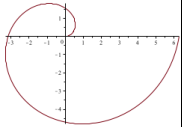
\includegraphics[width=0.3\textwidth]{spiral.pdf}

\prob{9}  A function $f$ is defined by a power series as
    $$f(x) = \sum_{n=0}^\infty \frac{(-1)^n}{(3^n) \sqrt{n+1}} (x-5)^n$$

\epart{a} Find the interval of convergence of the series.

\epart{b} Give numerical values of $f(5)$, $f'(5)$, and $f''(5)$.

\prob{10}  Determine whether the following series converge or diverge.  State what test you use, and show enough work to make clear that you have applied the test correctly.

\epart{a} $\ds \sum_{n=0}^\infty \frac{\sqrt{n}+1}{3n^2 + 1}$

\epart{b} $\ds \sum_{n=1}^\infty (-1)^n \frac{e^n}{n^2}$

\epart{c} $\ds \sum_{n=1}^\infty \frac{7^n}{(n+1)!}$

\epart{d} $\ds \sum_{n=1}^\infty (-1)^n \frac{1}{\sqrt{n+2}}$

\end{document}
